\section{Data}
\label{sec:data}

The Nottingham Music Database \cite{NMD} is encoded in \ABC notation, which is musical notation in text format \cite{ABC}.
An example of \ABC notation can be seen at the top of Figure~\ref{fig:data:features}.
It includes a total of $1034$ folk tunes divided into nine different collections based genres or composers.
The folk tunes are separated into a training set of $659$ tunes, validation set of $165$ tunes, and a test set of $207$ tunes. Three tunes were omitted due to bad formatting.

To use the tunes in the models,
the tunes are first converted from the \ABC format to melodies with notes and rests.
Then the pitches and duration are extracted from the sequence of notes and rests and put into a pitch sequence and a duration sequence, respectively.
Rests are represented in the pitch sequence by a $0$.
Finally, both sequences are one-hot encoded, which results in $35$ pitch values and $14$ duration values.
An end-of-sequence character has also been included in both sequences.
This preprocessing is illustrated in Figure~\ref{fig:data:features}.

\begin{figure}
	\centering
	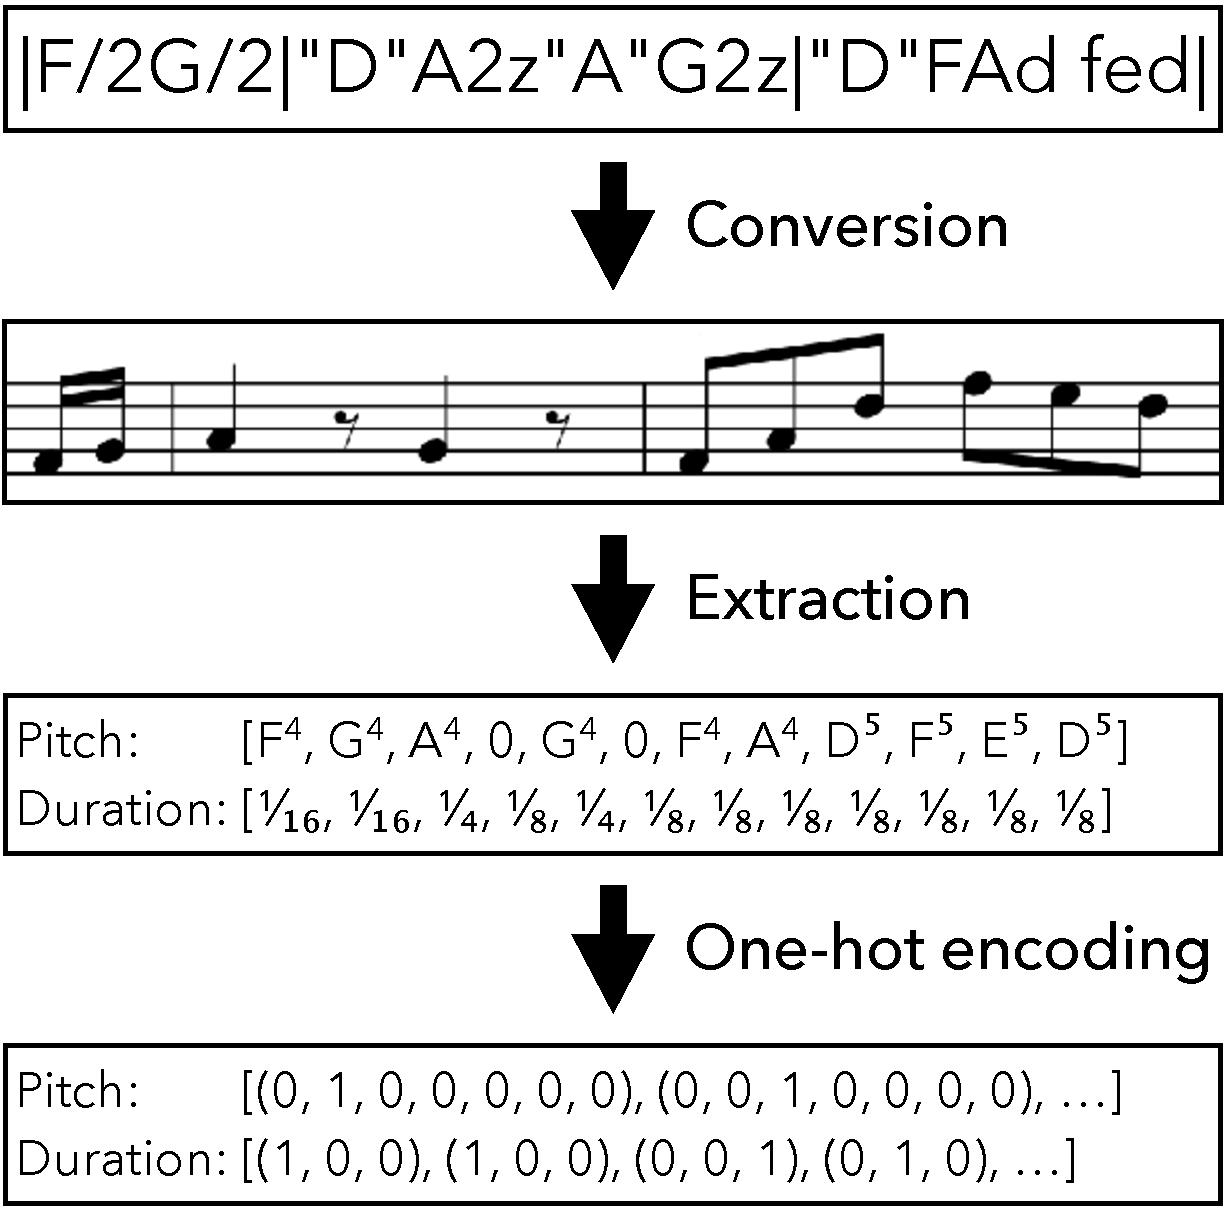
\includegraphics[width=0.8\linewidth]{Features}
	\caption{Extraction of pitch and duration sequences from \ABC notation.}
	\label{fig:data:features}
\end{figure}
